\documentclass[conference]{IEEEtran}
\usepackage{cite}
\usepackage{amsmath,amssymb,amsfonts}
\usepackage{algorithmic}
\usepackage{graphicx}
\usepackage{textcomp}
\usepackage{xcolor}
\usepackage{float}
\usepackage{booktabs}
\setlength{\floatsep}{0pt}
\setlength{\intextsep}{0pt}

\def\BibTeX{{\rm B\kern-.05em{\sc i\kern-.025em b}\kern-.08em
    T\kern-.1667em\lower.7ex\hbox{E}\kern-.125emX}}
\begin{document}

\title{Financial Statement Fraud Detection Using Large Language Models}

\author{\IEEEauthorblockN{Ryan Huang}\IEEEauthorblockA{\textit{Department of Computer Science}\\\textit{Department of Economics}\\\textit{UNC Chapel-Hill}\\Chapel Hill, USA\\rhuang1@unc.edu}\and
\IEEEauthorblockN{Chunjiang Zhu}
\IEEEauthorblockA{\textit{Department of Computer Science} \\
\textit{UNC Greensboro}\\
Greensboro, USA \\
c\_zhu3@uncg.edu}
\and
\IEEEauthorblockN{Qianqian Tong}
\IEEEauthorblockA{\textit{Department of Computer Science} \\
\textit{UNC Greensboro}\\
Greensboro, USA \\
q\_tong@uncg.edu}
\and
}

\maketitle

\begin{abstract} We develop a new fraud detection model incorporating recent technological advances in Large Language Models such as LLaMA3 and GPT-4o. We demonstrate that combining deep learning knowledge with domain knowledge benefits fraud detection. We differ from previous research by using large language models to analyze financial, textual, and linguistic data from annual 10-k financial statements.
\end{abstract}

\begin{IEEEkeywords}
Fraud Detection, Large Language Models, Machine Learning
\end{IEEEkeywords}

\section{Introduction}
Fraud is a global issue that spans various industries, and when left unchecked, it can cause serious harm to stakeholders, employees, and other affiliates. Financial fraudulent activities worldwide have amounted to \$5.127 trillion, with most of the increase in the past ten years \cite{b5}. However, with the rise of artificial intelligence usage in businesses in the past five years, that number is almost certain to rise further and cause more damage. Financial statement fraud, however, is challenging to detect and prevent. Typically, there are 40-50 cases a year and even those that are detected end up being detected years after the fraud had been committed \cite{b4}. Standard machine learning models have proven to have good accuracy but need to catch up in correctly predicting the right firms to be fraudulent. With recent technological advances in large language models, more effective methods would be invaluable to regulators, auditors, and investors. \newline\indent Our study aims to develop a new dataset and new financial statement fraud detection model using available information from the SEC financial statements and the Accounting and Auditing Enforcement Releases (AAERs). We differ from Bao et al. in that we do not limit ourselves to only financial data. We will model our model after Chen, Kelly, and Xiu \cite{b2}. They leverage the LLMs such as GPT and LLaMA to analyze all news data to predict stock returns. In the scope of this study, there is little existing literature on using LLMs to analyze financial text, voice, and facial expression data. We provide an implementation using LLMs to improve on existing machine learning results. Similarly to Bao et al., we seek to explain fraud out-of-sample, essentially making this a prediction problem, rather than the standard causal inference problem such as in Dechow et al. \cite{b3}. \newline\indent We use five types of fraud prediction models from previous literature as benchmarks: logistic regression, random forest, SVM, XGBoost, and RUSBoost. We use similar performance evaluation metrics as Bao et al. \cite{b7} to assess the performance of these models. These will be discussed in section IV of the paper. First, we use the area under the Receiver Operating Characteristics (ROC) curve (AUC). We also use the Normalized Discounted Cumulative Gain at the position $k$ (NDCG\@k). Thirdly, we modify our measures of sensitivity and precision to reflect the top 1\% of predicted fraudulent companies probability. \newline\indent An exciting question is whether adding more features to our models will improve the performance. Once the LLM is implemented, we must re-evaluate existing machine learning models with the new data. We will also perform a more in-depth analysis of the most important financial variables and ratios based on more current literature. With only 28 financial variables and 14 financial ratios, we do not see the performance increasing significantly unless more information is given about the companies (i.e., MD\&A, earnings call data, etc.). Our study will join an extremely small area of financial literature incorporating LLMs to predict financial statement fraud out of sample. Studies like Chen, Kelly, Xiu \cite{b2} have paved the way for using LLMs in financial research. Some of the preliminary results raise the possibility that the LLMs could further improve the precision of machine learning models in fraud detection in financial statements. 

\section{Background}

One of the most common accounting principles is the fraud triangle, proposed by Cressey in the 1970s. It consists of three components: perceived financial need, opportunity, and rationalization \cite{b8}. Most companies expect significant returns while putting in the minimum effort to maximize their scarce resources. Fraudulent activities are often only discovered after whistleblower tips to the SEC. While fraudulent activities may seem one-dimensional on the surface, there are many indirect costs associated with fraud, including loss of reputation, productivity loss, and irreversible financial damage to employees of the firm that is committing fraud. 

\section{Methodology} We use several machine learning methods outlined in Bao et al. \cite{b7} and choose other common methods to experiment on fraud datasets. We adjust the hyper-parameters to tune the model performance. We use the public dataset from Bao et al. \cite{b7} and conduct our baseline analysis on their data. For the initial testing year 2003, we used 1991-2001 as the training set and 2002 as a validation set to tune our models. For each additional year after 2003 up until our last sample test year of 2008, we increase the training and validation sets by one year to increase model performance. For example, for the test year 2008, we use 1991-2006 as the training set, and validate on 2007. Dyck, Morse, and Zingales \cite{b4} find it takes, on average, two years for fraudulent activities to be discovered, hence the two-year gap between the training set and test set. Additionally, we set the $random\_state$ to be 42 for ease of recreatibility. We also normalize the features for easier interpretability. Fig. 1 shows the overall methodology for our experiment. \vspace{10pt} \begin{figure}[H]
\centerline{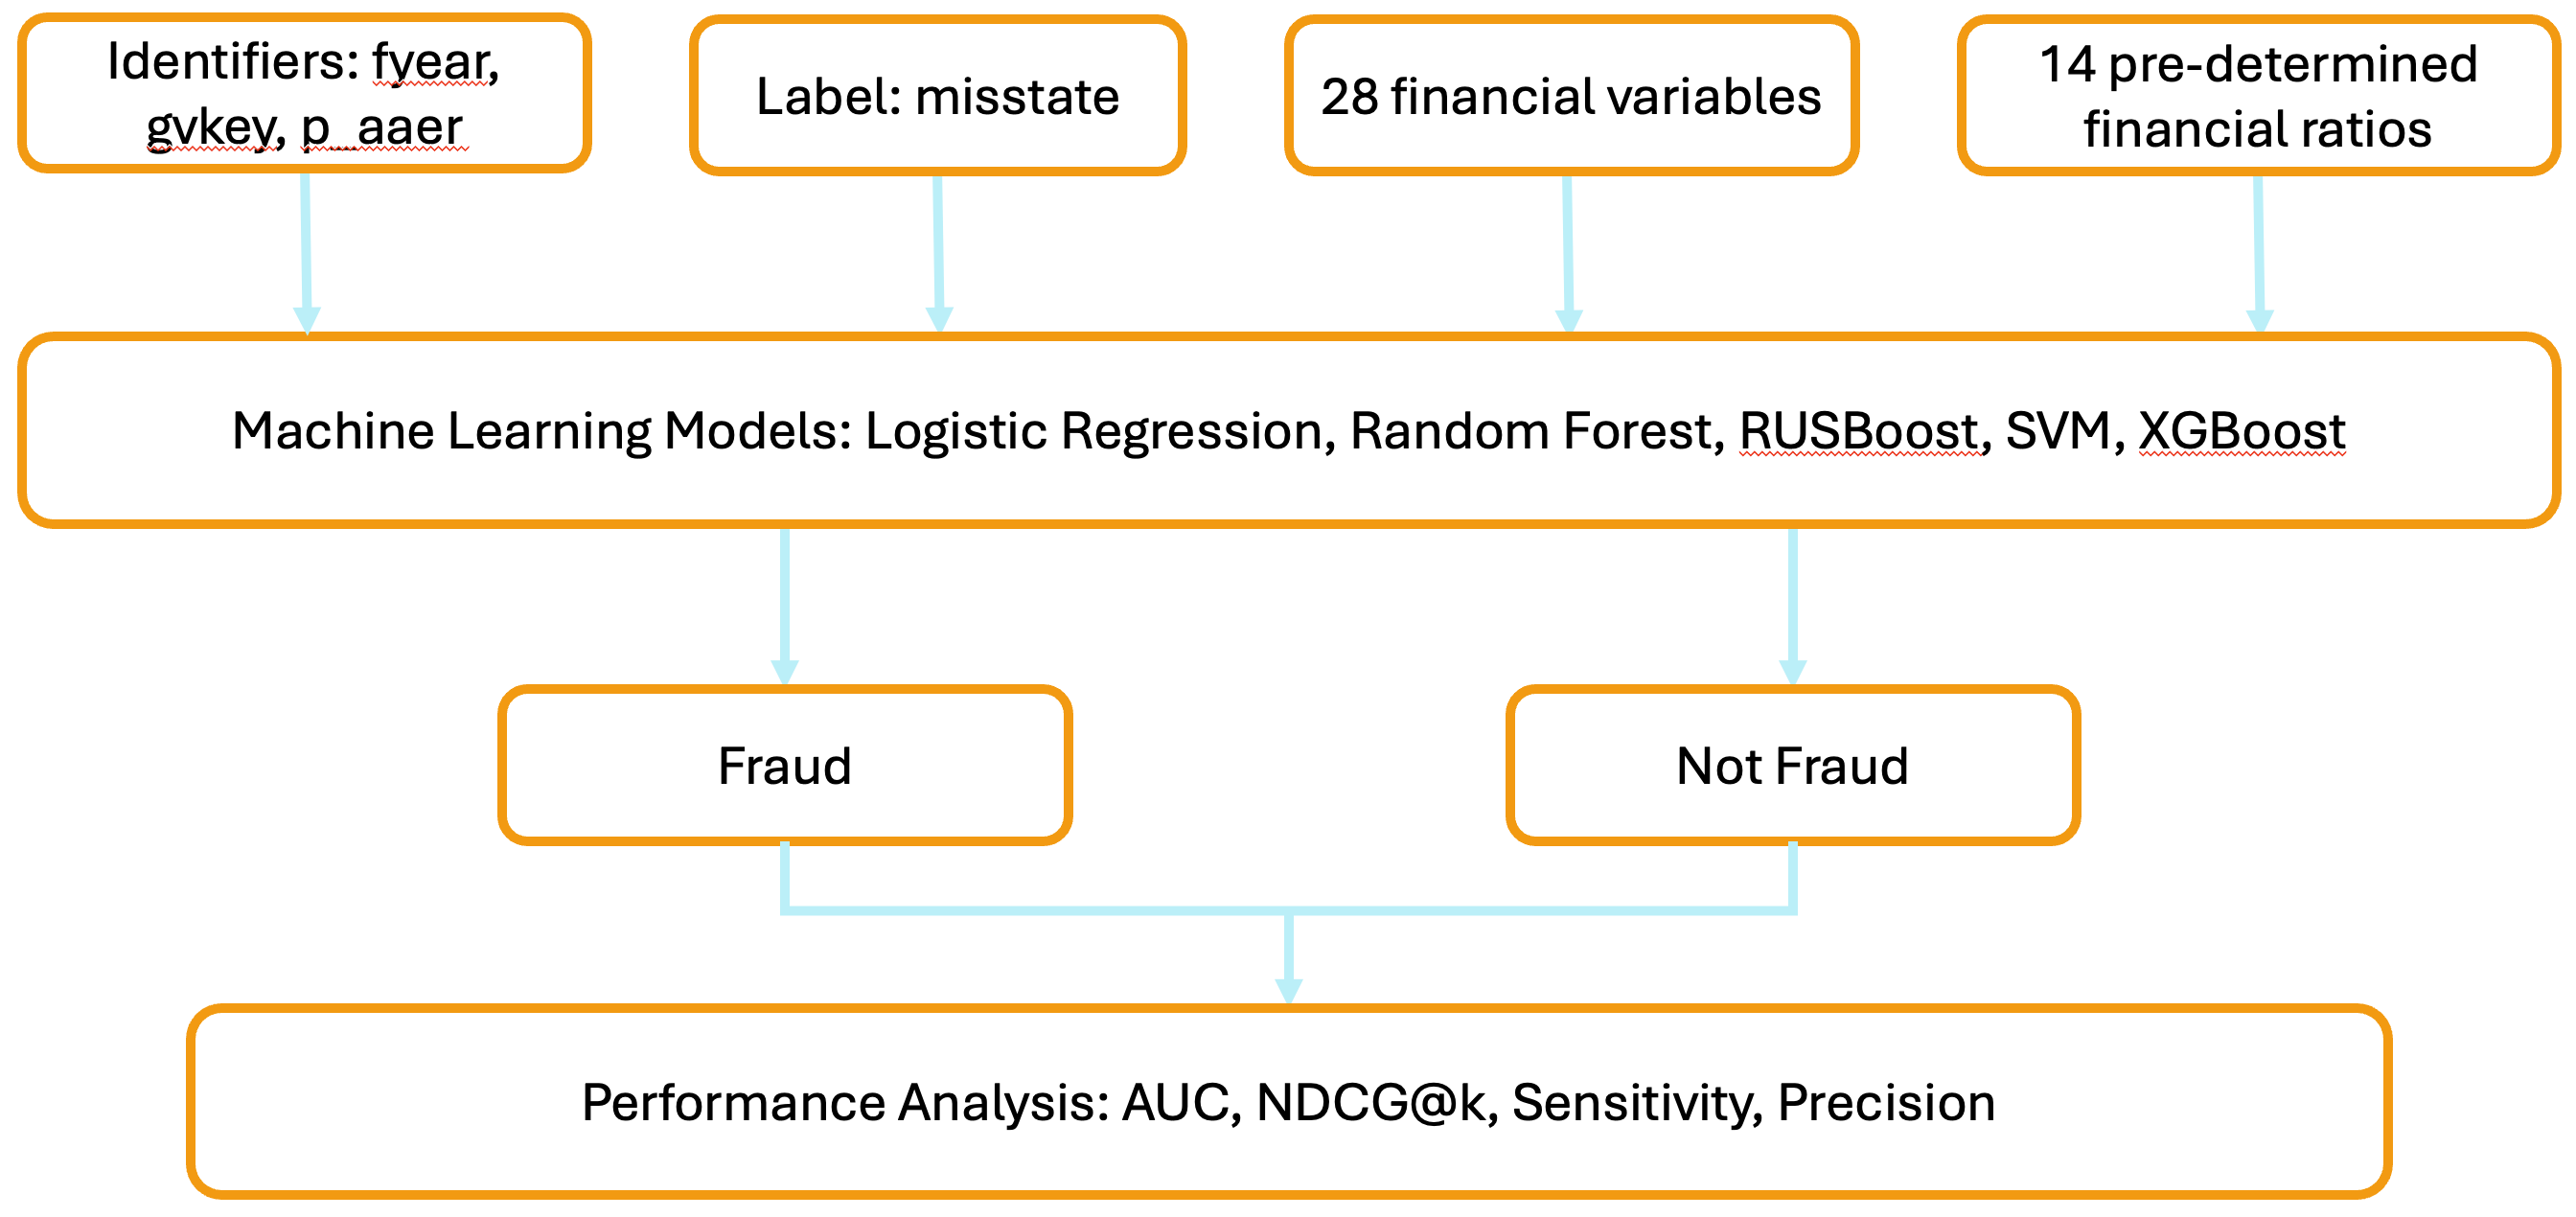
\includegraphics[width=\columnwidth]{mlmethod}}
\caption{Figure of Experiment}
\label{fig}
\end{figure}
\vspace{10pt}We describe the parameters of our experiments below:\subsection{Machine Learning Methods} 
\subsubsection{Logistic Regression} We leverage the standard logistic regression model to predict fraud probabilities. We employ a class weight ratio to deal with the imbalance in the dataset, calculated by taking the ratio of fraudulent instances to non-fraudulent instances. We then pick those firms above a threshold and classify them as fraudulent. 
\subsubsection{Random Forest} We use a standard Random Forest classifier by tuning the following hyper-parameters: $n\_estimators, class\_weight,$ and $max\_depth$. We use the validation set and GridSearch to find the optimal parameters that maximize AUC. We employ the same class weight ratio from logistic regression to handle imbalanced data.
\subsubsection{SVM} We optimize our SVM model by picking a C, which is the cost ratio of misclassifying fraud and non-fraud. The financial kernel from Cecchini et al. \cite{b1} takes advantage of the raw financial data by mapping it into pre-defined ratios, typically intrayear and year-to-year change ratios. We choose not to use it because of the difficulty of implementation and the lack of performance gains over the standard SVM model.
\subsubsection{XGBoost} Similar to Random Forest, we perform a GridSearch for the optimal parameters. We optimize for AUC by adjusting $max\_depth, learning\_rate,$ and $n\_estimators$, where $learning\_rate$ scales the prediction of each weak learner. 
\subsubsection{RUSBoost} We use the random undersampling package in Python to undersample the majority class so that the input is a matched set of fraud and non-fraudulent observations. We train the matched sample through a weak classifier, which will give a correct or incorrect classification. If the weak classifier is incorrect, the weight of the incorrect observation will be increased and vice versa. Once we iterate over and over, we apply a error rate-based weight on each weak classifier and take a weighted average to build a strong classifier to predict. This is depicted in Fig. 2: \begin{figure}[H] \vspace{10pt}
\centerline{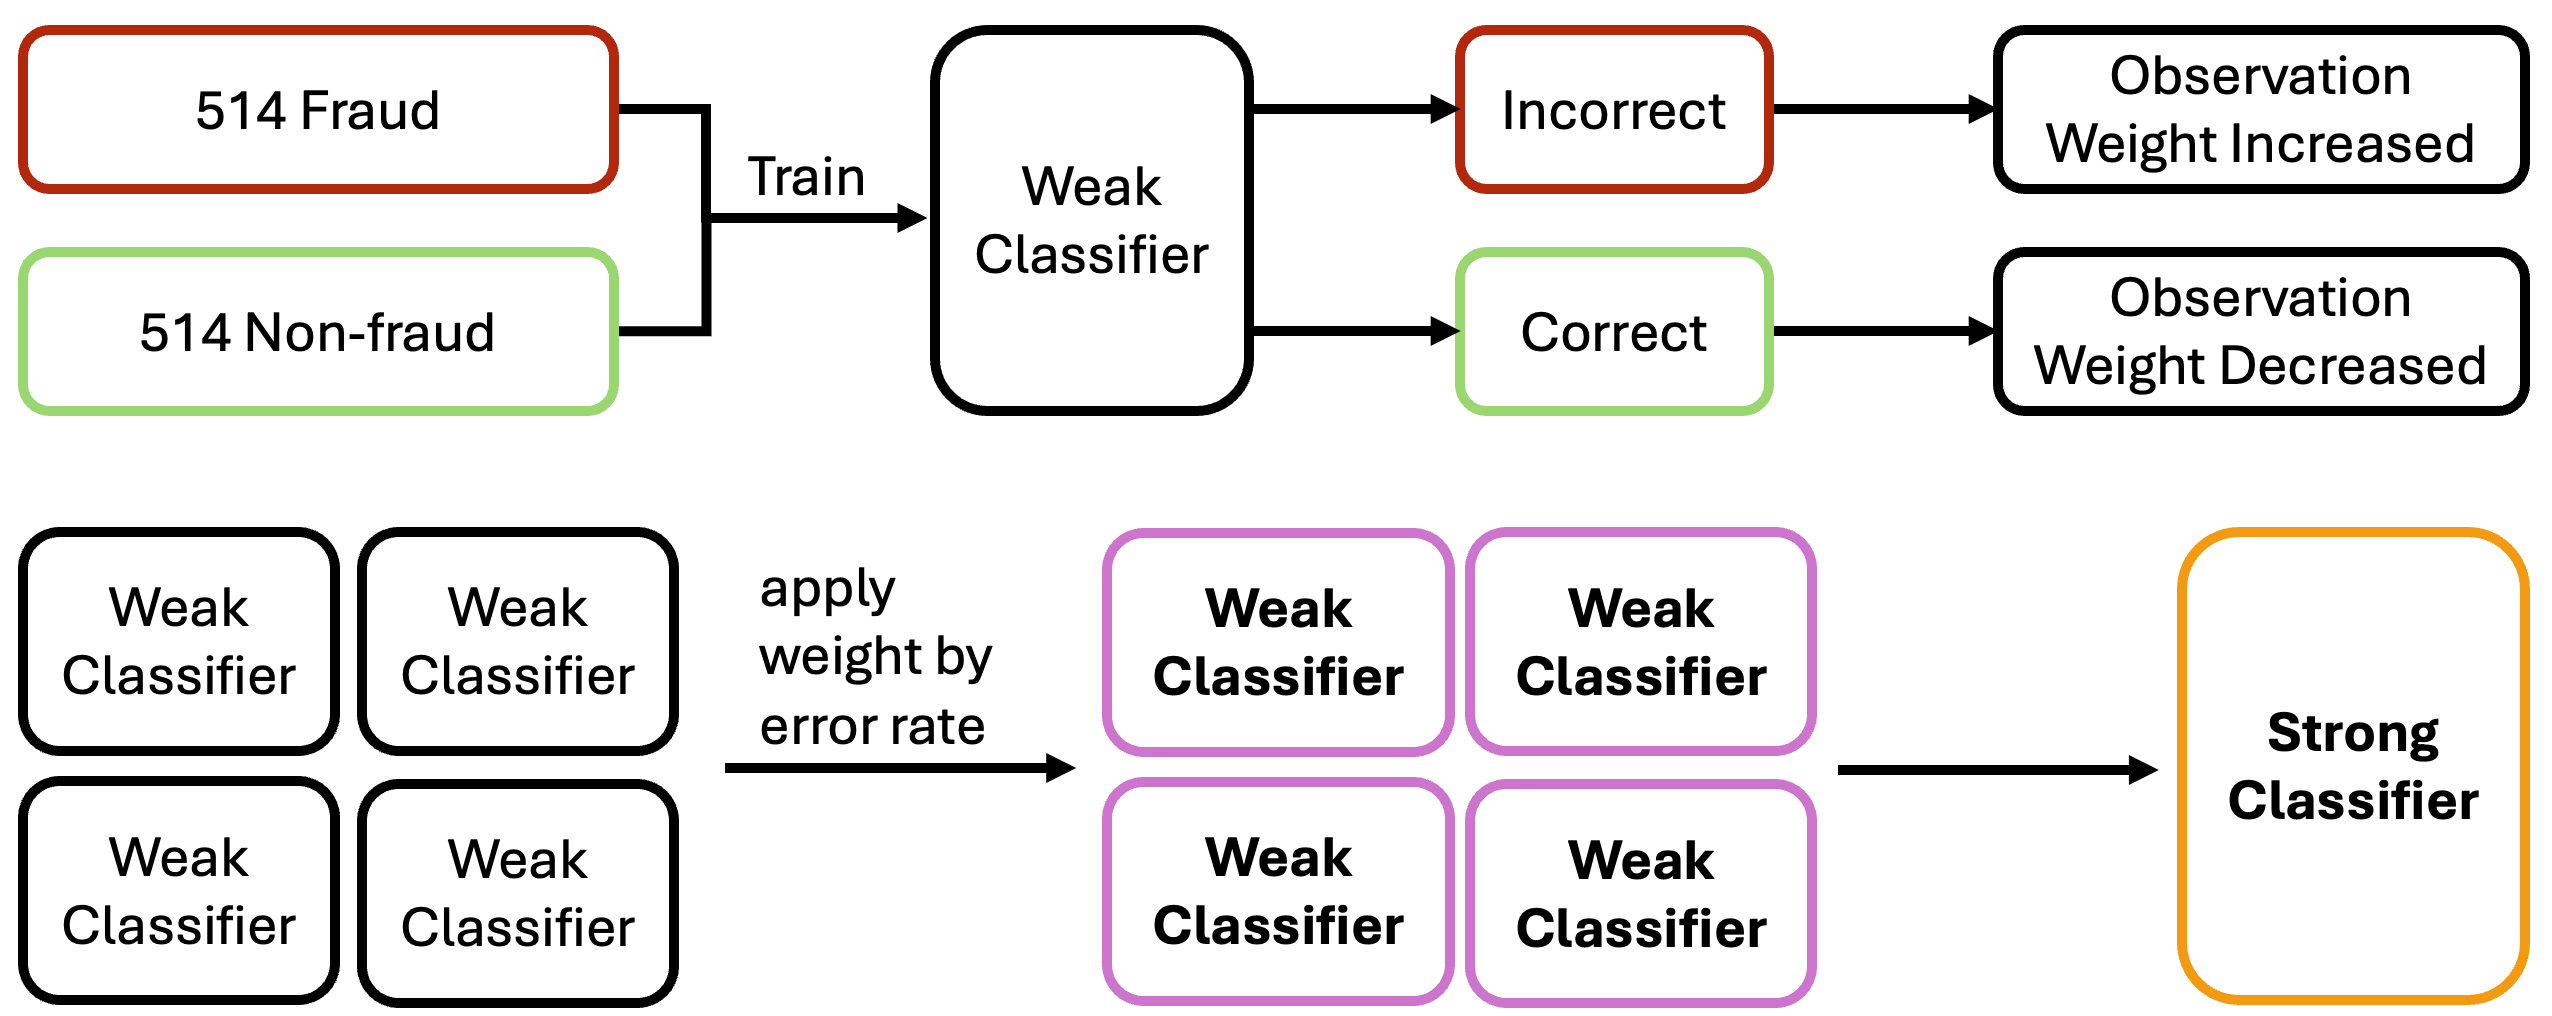
\includegraphics[width=\columnwidth]{rusboost}}
\caption{Depiction of RUSBoost model. The top half repeats itself, and the bottom half takes a weighted average of all the weak classifiers from the top.}
\label{fig}
\end{figure} \vspace{10pt}
\section{Data}
We use the public dataset compiled from Detecting Accounting Fraud in Publicly Traded U.S. Firms Using a Machine Learning Approach. We will refer to this dataset as the JAR dataset in the rest of the paper. They use financial data from Compustat to create the dataset. The dataset consists of two unique identifier variables for each firm: $fyear$ and $gvkey$. The $gvkey$, or Global Company Key, is a six-digit code assigned to each firm in the Compustat database.  For the fraud label, they track the case number from the SEC AAER database, which contains a list of all firms that have been audited or investigated for fraud. This is represented by $p\_aaer$ in the public dataset, and for every instance of a case number, the label we are predicting, $misstate$, is equal to one. The main features of the public dataset consist of a pairing of 28 financial variables with 14 financial ratios. As the paper we are basing our study on is from 2019, the dataset only consists of cases up until 2018 and needs to be completed. However, we only used the 1991-2008 sample period for our initial testing. The sample began in 1991 due to the stricter enforcement of accounting fraud. The sample ends in 2008 due to the reduction of accounting fraud enforcement due to the higher probability of accounting fraud cases going undetected post-2008 \cite{b6}.  

\subsection{Data Distribution}
The total number of fraud instances in the JAR dataset is 964, and the total number of non-fraudulent instances is 145,081, summing up to 146,045 entries total. We also plot the distribution of the number of fraud cases per year and find that it follows a relatively normal distribution with a peak in fraud cases in the 2000-2003 range. When we look at the unique number of fraud cases per year, we find that the shape of the distribution of fraud cases per year is similar, but there are significantly fewer cases in the peak years (2000-2003). Table I displays the most common offenders within the dataset. Figure III shows the number of fraud cases per year with the number of total fraud cases overlapping the number of unique fraud cases per year. \vspace{10pt}
\begin{figure}[htbp]
\centerline{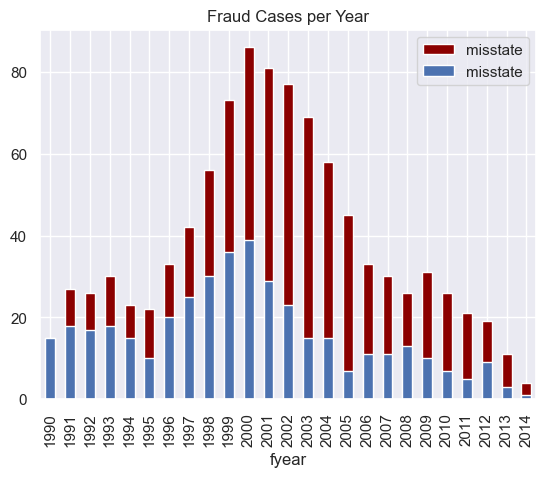
\includegraphics[width=\columnwidth]{fraudoverlap}}
\caption{The blue bars are new cases for every year, and the red bars represent the total number of fraud cases, including repeat offenders.}
\label{fig}
\end{figure} \vspace{10pt}
\begin{table}[H]
\caption{Repeat Offenders Frequency}
\centering
\begin{tabular}{@{}p{6.3cm}p{2.1cm}@{}} 
\toprule
\textbf{\hspace{5mm}Company Name} & \textbf{Frequency}\hspace{5mm} \\
\midrule
\hspace{5mm}Black Box Corp & 13\hspace{5mm} \\
\hspace{5mm}Overseas Shipholding Group & 12\hspace{5mm} \\
\hspace{5mm}Affiliated Computer Services & 12\hspace{5mm} \\
\hspace{5mm}UnitedHealth Group Inc & 11\hspace{5mm} \\
\hspace{5mm}Integrated Silicon Solution & 9\hspace{5mm} \\
\hspace{5mm}Mercury Interactive Corp & 9\hspace{5mm} \\
\hspace{5mm}Monster Worldwide Inc & 8\hspace{5mm} \\
\hspace{5mm}Broadcom Corp -Cl A & 8\hspace{5mm} \\
\hspace{5mm}Vitesse Semiconductor Corp & 8\hspace{5mm} \\
\hspace{5mm}Comverse Technology Inc & 7\hspace{5mm} \\
\hspace{5mm}Elbit Medical Imaging Ltd & 7\hspace{5mm}  \\
\hspace{5mm}Conagra Foods Inc & 7\hspace{5mm} \\
\hspace{5mm}Interpublic Group of Cos & 7\hspace{5mm} \\
\hspace{5mm}NCI Inc & 7\hspace{5mm} \\
\hspace{5mm}Analogic Corp & 6\hspace{5mm} \\
\hspace{5mm}Dow Chemical & 6\hspace{5mm} \\
\hspace{5mm}Take-Two Interactive Sftwr & 6\hspace{5mm} \\
\hspace{5mm}Diebold Inc & 6\hspace{5mm} \\
\hspace{5mm}NIC Inc & 6\hspace{5mm} \\
\hspace{5mm}Engineered Support Systems & 6\hspace{5mm} \\
\hspace{5mm}Cummins Inc & 6\hspace{5mm} \\
\hspace{5mm}UCI Medical Affiliates Inc & 6\hspace{5mm} \\
\hspace{5mm}Brooks Automation Inc & 6\hspace{5mm} \\
\bottomrule
\end{tabular}
\label{tab1}
\end{table} \vspace{10pt}\subsection{Features}
We use a list of raw financial variables selected by Bao et al. \cite{b7} based on Cecchini et al. \cite{b1} and Dechow et al. \cite{b3}, compiled from the Compustat database. The final dataset from Bao et al., which we use in this study for a baseline, contains 28 financial variables and 14 financial ratios, which are abbreviated for convenience in Table II and III: \vspace{10pt}

\label{AA}
\begin{table}[htbp]
\caption{28 Financial Variables}
\centering
\begin{tabular}{@{}p{3.4cm}p{5cm}@{}} 
\toprule
\textbf{\hspace{5mm}Abbreviation} & \textbf{Financial Variable\hspace{5mm}} \\
\midrule
\hspace{5mm}ACT & Current Assets, Total\hspace{5mm} \\
\hspace{5mm}AP & Accounts Payable Trade\hspace{5mm} \\
\hspace{5mm}AT & Assets, Total\hspace{5mm} \\
\hspace{5mm}CEQ & Common/Ordinary Equity, Total\hspace{5mm} \\
\hspace{5mm}CHE & Cash and Short-Term Investments\hspace{5mm} \\
\hspace{5mm}COGS & Cost of Goods Sold\hspace{5mm} \\
\hspace{5mm}CSHO & Common Shares Outstanding\hspace{5mm} \\
\hspace{5mm}DLC & Debt in Current Liabilities, Total\hspace{5mm} \\
\hspace{5mm}DLTIS & Long-Term Debt Insurance\hspace{5mm} \\
\hspace{5mm}DLTT & Long-Term Debt, Total\hspace{5mm} \\
\hspace{5mm}DP & Depreciation and Amortization\hspace{5mm} \\
\hspace{5mm}IB & Income Before Extraordinary Items\hspace{5mm} \\
\hspace{5mm}INVT & Inventories, Total\hspace{5mm} \\
\hspace{5mm}IVAO & Investments Advances, Other\hspace{5mm} \\
\hspace{5mm}IVST & Short Term Investments, Total\hspace{5mm} \\
\hspace{5mm}LCT & Current Liabilities, Total\hspace{5mm} \\
\hspace{5mm}LT & Liabilities, Total\hspace{5mm} \\
\hspace{5mm}NI & Net Income (Loss)\hspace{5mm} \\
\hspace{5mm}PPEGT & Property, Plant, and Equipment, Total\hspace{5mm} \\
\hspace{5mm}PSTK & Preferred/Preference Stock (Capital), Total \\
\hspace{5mm}RE & Retained Earnings\hspace{5mm} \\
\hspace{5mm}RECT & Receivables, Total\hspace{5mm} \\
\hspace{5mm}SALE & Sales/Turnover (Net)\hspace{5mm} \\
\hspace{5mm}SSTK & Sale of Common and Preferred Stock\hspace{5mm} \\
\hspace{5mm}TXP & Income Taxes Payable\hspace{5mm} \\
\hspace{5mm}TXT & Income Taxes, Total\hspace{5mm} \\
\hspace{5mm}XINT & Interest and Related Expense, Total\hspace{5mm} \\
\hspace{5mm}PRCC\_F & Price Close, Annual, Fiscal\hspace{5mm} \\
\bottomrule
\end{tabular}
\label{tab1}
\end{table}
\vspace{10pt}
\begin{table}[htbp]
\caption{14 Financial Ratios}
\centering
\begin{tabular}{@{}p{2.3cm}p{6.1cm}@{}} 
\toprule
\textbf{\hspace{5mm}Abbreviation} & \textbf{Financial Variable\hspace{5mm}} \\
\midrule
\hspace{5mm}DCH\_WC & WC Accruals\hspace{3mm} \\
\hspace{5mm}CH\_RSST & RSST Accruals\hspace{3mm} \\
\hspace{5mm}DCH\_REC & Change in Receivables\hspace{5mm} \\
\hspace{5mm}DCH\_INV & Change in Inventory\hspace{5mm} \\
\hspace{5mm}SOFT\_ASSET & \% Soft Assets \hspace{5mm} \\
\hspace{5mm}DPI & Depreciation Index\hspace{5mm} \\
\hspace{5mm}CH\_CS & Change in Cash Sales\hspace{5mm} \\
\hspace{5mm}CH\_CM & Change in Cash Margin\hspace{5mm} \\
\hspace{5mm}CH\_ROA & Change in Return on Assets\hspace{5mm} \\
\hspace{5mm}CH\_FCF & Change in Free Cash Flows\hspace{5mm} \\
\hspace{5mm}REOA & Retained Earnings Over Total Assets\hspace{5mm} \\
\hspace{5mm}EBIT & Earnings Before Interest and Taxes Over Total Assets \\
\hspace{5mm}ISSUE & Actual Issuance\hspace{5mm} \\
\hspace{5mm}BM & Book-to-Market\hspace{5mm} \\
\bottomrule
\end{tabular}
\label{tab1}
\end{table} \vspace{10pt}


\section{Performance Evaluation Metrics}

Due to the imbalance of our dataset, running standard machine learning methods will result in many false positives. Similarly, if we consider the reality, auditors cannot and will not audit every company. That would take too many resources, and even then, they still may not be accurate in detecting fraud. Therefore, we use the AUC, Precision, Sensitivity, and NCDG@k as defined below from Bao et al. \vspace{10pt}\begin{figure}[!htbp]
	\centerline{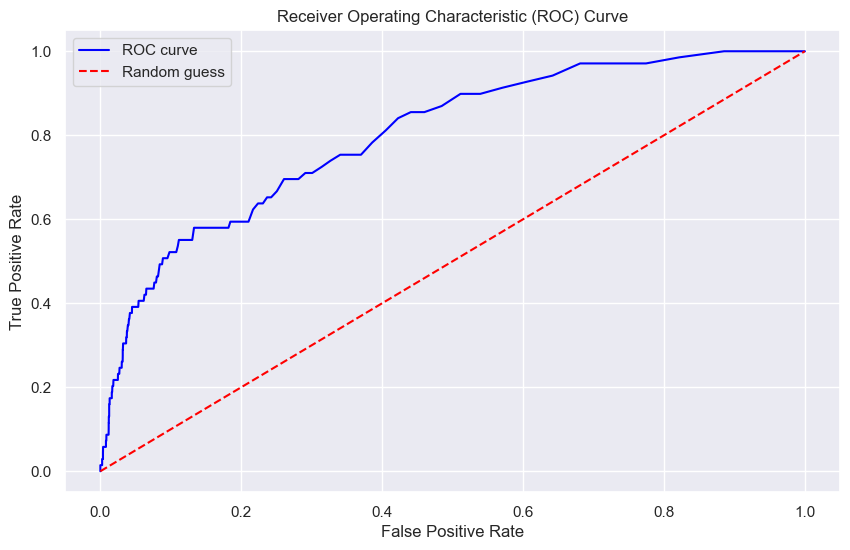
\includegraphics[width=\columnwidth]{roc}}
	\caption{ROC curve for Random Forest, Test Year = 2003}
	\label{fig}
	\end{figure}\vspace{10pt}\subsubsection{AUC} The standard performance metric is accuracy which is defined as $\frac{TP+TN}{TP+FN+FP+TN}$, where $TP$ is when the model correctly classifies the firm as a fraud; $TN$ is when the model correctly classifies the firm as non-fraudulent; $FP$ is when the model classifies a firm as fraudulent, but it is not; and $FN$ is when the model does not classify a firm as fraudulent when it should be. On the other hand, AUC relies on the true and false positive rates, such as the ROC curve, which shows a classifier's performance at a certain threshold. In our study, anything below 0.5 should not be feasible since a random guess results in an AUC of 0.5. On the other hand, a perfect AUC is 1.0 and should be very rare. The AUC is the probability that the classifier will rank a true positive higher than a non-fraudulent firm \cite{b9}. As shown in Fig. 4, our random forest model performs quite well with an AUC of 0.8037. The optimal ROC curve is when the true positive rate is maximized, and the false positive rate is minimized.

	\subsubsection{NDCG@k} Bao et al. considers the fraud prediction task as a ranking problem. They use a discounted cumulative gain function to limit the out-of-sample performance evaluation to only the firms with the highest predicted probability of fraud. The DCG@k scores a fraudulent instance higher than a non-fraudulent instance. The DCG@k is then normalized by the ideal DCG@k, where the ideal is defined by all the true instances of fraud being ranked at the top. Formally, this is: \vspace{10pt}\begin{figure}[H]
	\centerline{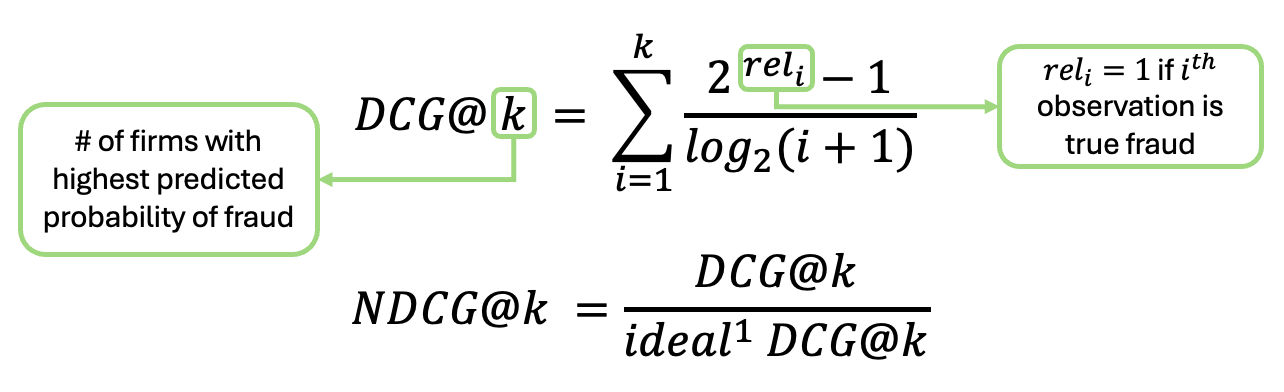
\includegraphics[width=\columnwidth]{ndcg}}
	\caption{Formula for DCG@k and NDCG@k}
	\label{fig}
	\end{figure} 
	\subsubsection{Sensitivity and Precision} From the NDCG@k, we also modify the sensitivity and precision metrics to follow the same methodology as NDCG@k. Rather than consider all the true positive firms, we consider only the top 1\% of firms with the highest predicted probability of committing fraud. This is more accurate for our results because of the imbalance of data. Formally, this is: \vspace{10pt}\begin{figure}[H]
	\centerline{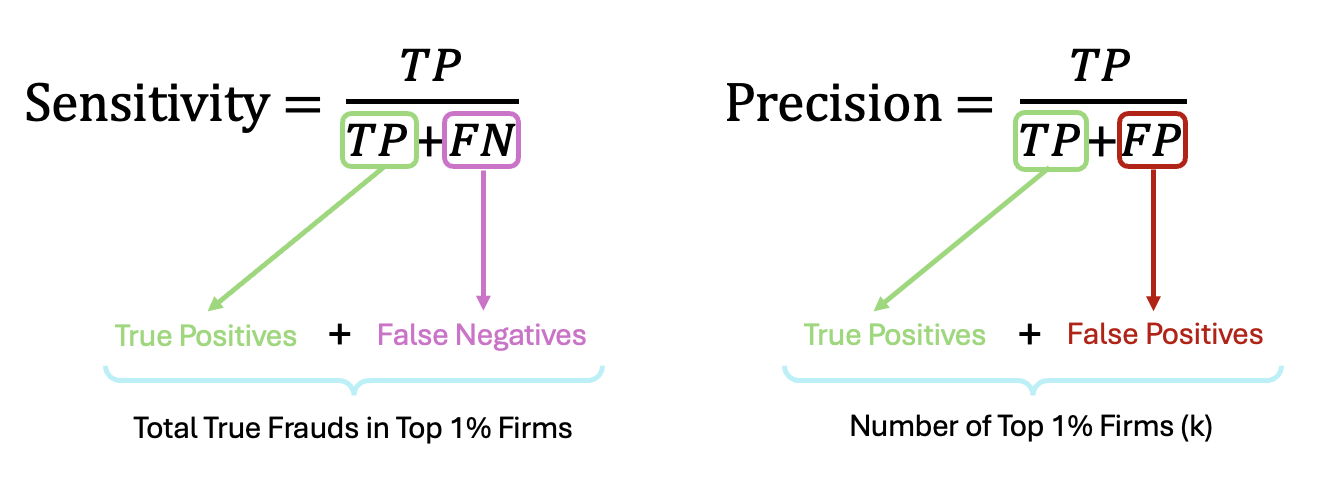
\includegraphics[width=\columnwidth]{sensprec}}
	\caption{Formula for Sensitivity and Precision}
	\label{fig}
	\end{figure} 
	\subsubsection{Comparing Improved Metrics with Standard Metrics} We compare the accuracy and AUC, sensitivity and modified sensitivity, and recall and modified recall. The figures below are from running the Random Forest model on 28 financial variables. The training set is the firms in the years 1991-2001, the validation set is 2002, and the test set is 2003. In Fig. 7, we find that accuracy is much more inflated than AUC, which naturally makes sense because a 1:150 imbalance has a less than one percent chance of incorrectly classifying a non-fraudulent firm. Once we delve deeper into the data, we can see in Fig. 8 that our number of true positives is relatively low, and our number of false positives is very high. When comparing the improved sensitivity to the standard sensitivity in Fig. 11, our figure shows un-interpretable values at one extreme or the other (0 or 1) and does not align with the confusion matrix (tp, fp, fn, tn). The modified sensitivity is interpretable as it aligns with our confusion matrix. Our precision displays the same behavior in Fig. 10. \newline\indent When looking at NDCG@k, sensitivity, and precision (improved metrics) in Fig. 9, the shape of the graphs shows a similar behavior. \vspace{15pt}
	\begin{figure}[H]
	\centerline{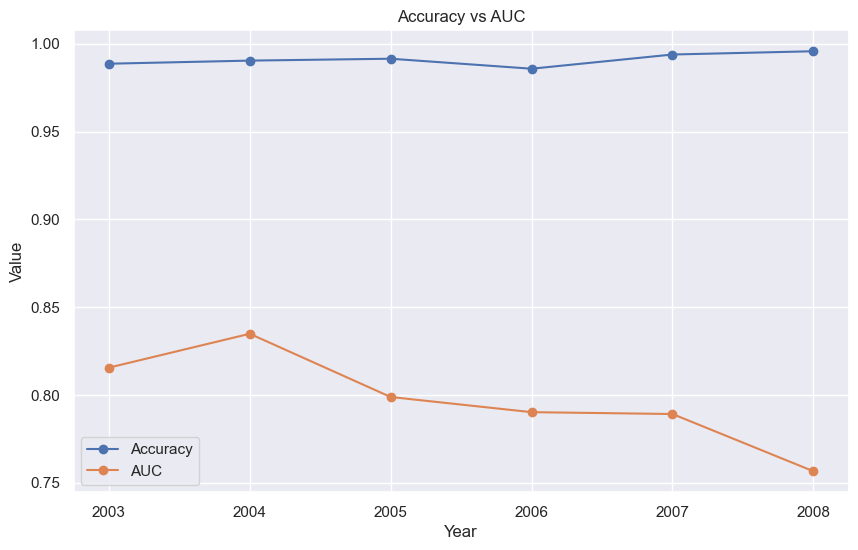
\includegraphics[width=\columnwidth]{output}}
	\caption{Accuracy vs AUC}
	\label{fig}
	\end{figure} \vspace{15pt}
		\begin{figure}[H]
	\centerline{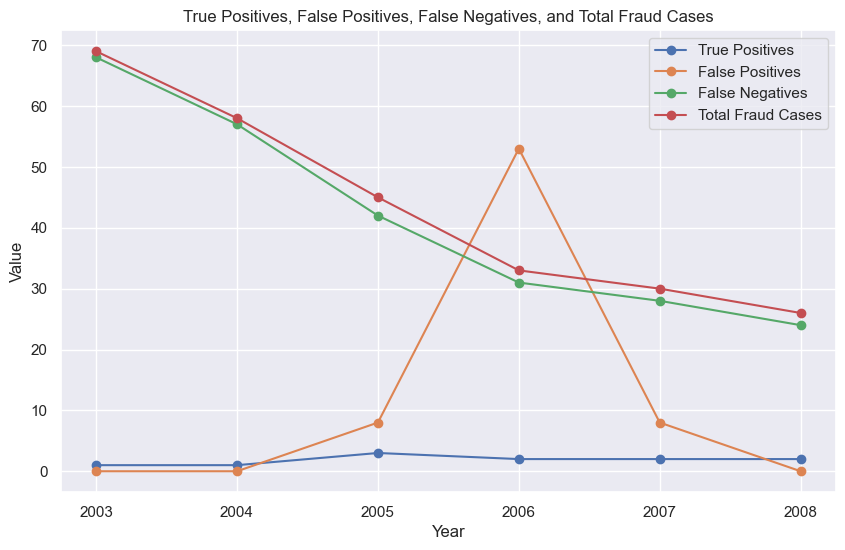
\includegraphics[width=\columnwidth]{output2}}
	\caption{\# of True Positives, False Positives, False Negatives, Total}
	\label{fig}
	\end{figure} \vspace{15pt}
			\begin{figure}[H]
	\centerline{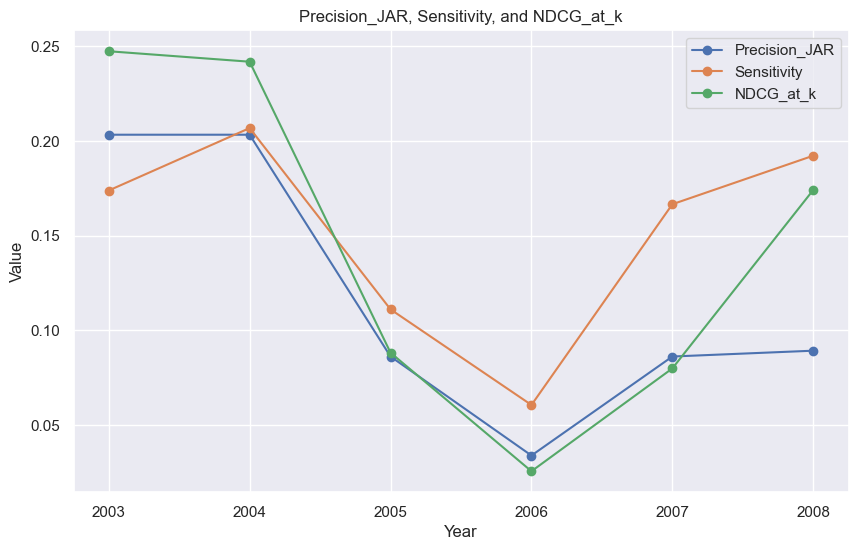
\includegraphics[width=\columnwidth]{output3}}
	\caption{Improved Performance Evaluation Metrics}
	\label{fig}
	\end{figure} \vspace{15pt}
				\begin{figure}[H]
	\centerline{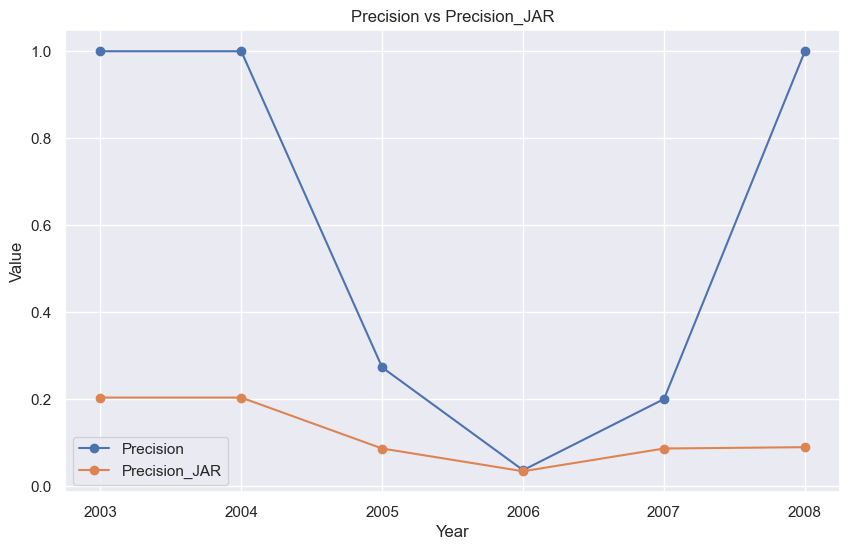
\includegraphics[width=\columnwidth]{output4}}
	\caption{Precision vs Precision (top 1\%)}
	\label{fig}
	\end{figure} \vspace{15pt}
					\begin{figure}[H]
	\centerline{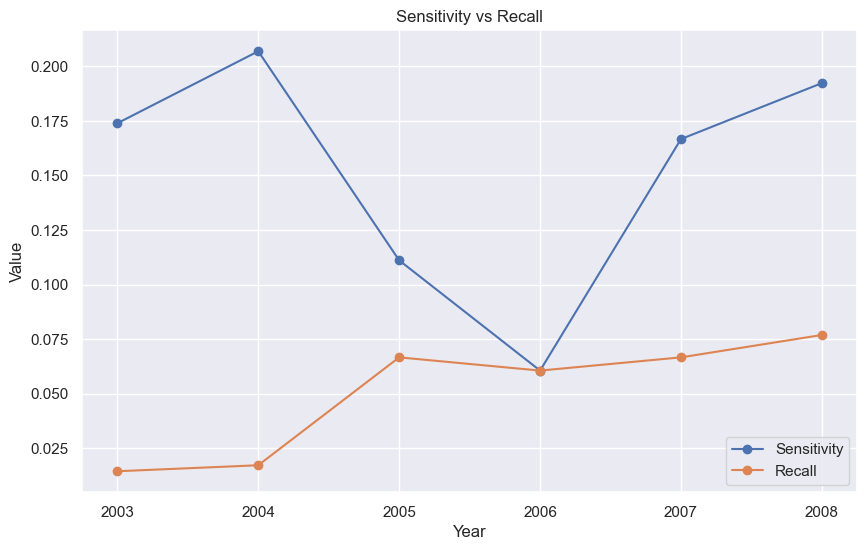
\includegraphics[width=\columnwidth]{output5}}
	\caption{Sensitivity (Recall for Top 1\%) vs Recall}
	\label{fig}
	\end{figure} \vspace{15pt}

\section{Preliminary Results} The preliminary results of our study, as shown in Tables IV-VII, provide an in-depth comparison of various machine learning methods applied to financial prediction tasks using different sets of input variables. By comparing methods across different input sets, we observe notable trends and patterns that shed light on the effectiveness of these techniques and the impact of additional financial ratios. The evaluation metrics considered are AUC (Area Under the Curve), NDCG@k (Normalized Discounted Cumulative Gain at rank k), Sensitivity, and Precision. \subsection{Bao et al. vs. our Results}Initially, the paper evaluates Logit, RUSBoost, and SVM using 28 financial variables. Among these, RUSBoost stands out with the highest AUC (0.725) and substantial improvements in sensitivity and precision. This suggests that RUSBoost, which balances class distributions through under-sampling, is particularly effective in handling the imbalanced nature of financial data, leading to more reliable predictions. Now compare this with our recreation. Table VII shows RUSBoost behaving similarly, with relatively little change in all performance metrics. Overall, we see slight differences in the AUC from our results and the results from Bao et al. However, when it comes to the other three metrics, we see they increase dramatically. We can attribute some of this increase to implementation differences, which we describe in detail how we leverage Logit and SVM to acquire the highest performance in all metrics. Expanding our methodology to include Random Forest and XGBoost in the second set of evaluations, we see significant enhancements in performance metrics: \begin{itemize} 
\item Random Forest emerges as the top performer with an AUC of 0.798 and superior sensitivity and precision. This indicates its robustness in capturing complex patterns and interactions within the financial data, making it a highly effective method.
\item XGBoost also demonstrates strong performance, though slightly trailing behind Random Forest. Its notable AUC and precision reflect its ability to handle large datasets with high dimensionality effectively \end{itemize}\subsection{Change in Input} When additional financial ratios are incorporated (Table VI), the performance of the models exhibits mixed results:\begin{itemize}
\item Random Forest maintains a high AUC but experiences reductions in other metrics. This indicates that while the additional ratios provide new information, they might also introduce noise or redundancy, slightly hindering the model’s sensitivity and precision.
\item XGBoost, on the other hand, shows a slight improvement in AUC, suggesting it can leverage the extra features to some extent, but like Random Forest, it faces a trade-off with sensitivity and precision. \end{itemize}\subsection{Main Takeaways} Overall, our preliminary finds underscore several key points: \begin{itemize} 
\item \textbf{Model Selection}: The choice of the machine learning method significantly impacts the performance. RUSBoost, Random Forest and XGBoost consistently outperform Logit and SVM, highlighting the benefits of ensemble methods and advanced boosting techniques in financial predictions.
\item \textbf{Feature Set Composition}: The introduction of additional financial ratios has a nuanced impact. While it can slightly enhance AUC, it often reduces sensitivity and precision. This suggests that while more features can provide more information, they also require careful selection and preprocessing to avoid diminishing returns or performance degradation due to overfitting or noise.
\item \textbf{Robustness and Adaptability}: Random Forest demonstrates robust performance across different feature sets, indicating its adaptability and ability to generalize well. In contrast, methods like Logit and SVM show more variability and are less robust to changes in the feature set.
\item \textbf{Sensitivity to Imbalanced Data}: Methods like RUSBoost, specifically address the class imbalance, show marked improvements in sensitivity and precision, critical for financial prediction tasks where the minority class (e.g., financial distress) is often of most significant interest.
 \end{itemize} These preliminary results highlight the importance of method selection and feature engineering in financial prediction. Ensemble methods, particularly Random Forest and RUSBoost, demonstrate superior performance and robustness while introducing additional financial ratios, which presents opportunities and challenges. Our future research will focus more on optimizing feature selection and exploring LLMs to introduce new features that may increase the performance of these models. 


\begin{table}[H]
\caption{Performance Evaluation Metrics for the Test Period 2003-08 \newline Input: 28 Financial Variables}
\centering
\begin{tabular}{p{2.495cm}cccc}
\toprule
\textbf{Method} & \textbf{AUC} & \textbf{NDCG@k} & \textbf{Sensitivity} & \textbf{Precision} \\
\midrule
\raggedright (1) Logit & 0.640 & 0.027 & 3.345\% & 2.845\% \\
\raggedright (2) Random Forest & 0.798 & 0.143 & 15.192\% & 11.706\% \\
\raggedright (3) RUSBoost & 0.770 & 0.051 & 4.963\% & 5.099\% \\
\raggedright (4) SVM & 0.638 & 0.024 & 3.057\% & 2.562\% \\
\raggedright (5) XGBoost & 0.760 & 0.099 & 9.634\% & 7.687\% \\
\bottomrule
\end{tabular}
\label{tab:performance}
\end{table}

\begin{table}[H]
\caption{Performance Evaluation Metrics for the Test Period 2003-08 \newline Input: 28 Financial Variables + 14 Financial Ratios}
\centering
\begin{tabular}{p{2.495cm}cccc}
\toprule
\textbf{Method} & \textbf{AUC} & \textbf{NDCG@k} & \textbf{Sensitivity} & \textbf{Precision} \\
\midrule
\raggedright (1) Logit & 0.703 & 0.022 & 3.103\% & 2.562\% \\
\raggedright (2) Random Forest & 0.790 & 0.084 & 7.689\% & 6.007\% \\
\raggedright (3) RUSBoost & 0.751 & 0.029 & 2.996\% & 2.835\% \\
\raggedright (4) SVM & 0.708 & 0.027 & 3.084\% & 2.285\% \\
\raggedright (5) XGBoost & 0.713 & 0.070 & 8.121\% & 6.546\% \\

\bottomrule
\end{tabular}
\end{table}



\begin{table}[H]
\caption{Percentage Change From Table IV to Table V}
\centering
\begin{tabular}{p{2.295cm}cccc}
\toprule
\textbf{Method} & \textbf{AUC} & \textbf{NDCG@k} & \textbf{Sensitivity} & \textbf{Precision} \\
\midrule
\raggedright (1) Logit & 9.84\% & -18.52\% & -9.95\% & -7.24\% \\
\raggedright (2) Random Forest & -1.00\% & -41.26\% & -48.68\% & -49.39\% \\
\raggedright (3) RUSBoost & -2.47\% & -43.14\% & -44.40\% & -39.63\% \\
\raggedright (4) SVM & 10.97\% & 12.50\% & -10.81\% & 0.88\% \\
\raggedright (5) XGBoost & -6.18\% & -29.29\% & -14.84\% & -15.71\% \\
\bottomrule
\end{tabular}
\label{tab:performance}
\end{table} \vspace{0.1pt}

\section{Next Steps} We present an updated visualization to Fig. 1 with the implementation of LLMs in our next steps. \vspace{15pt}\begin{figure}[H]
	\centerline{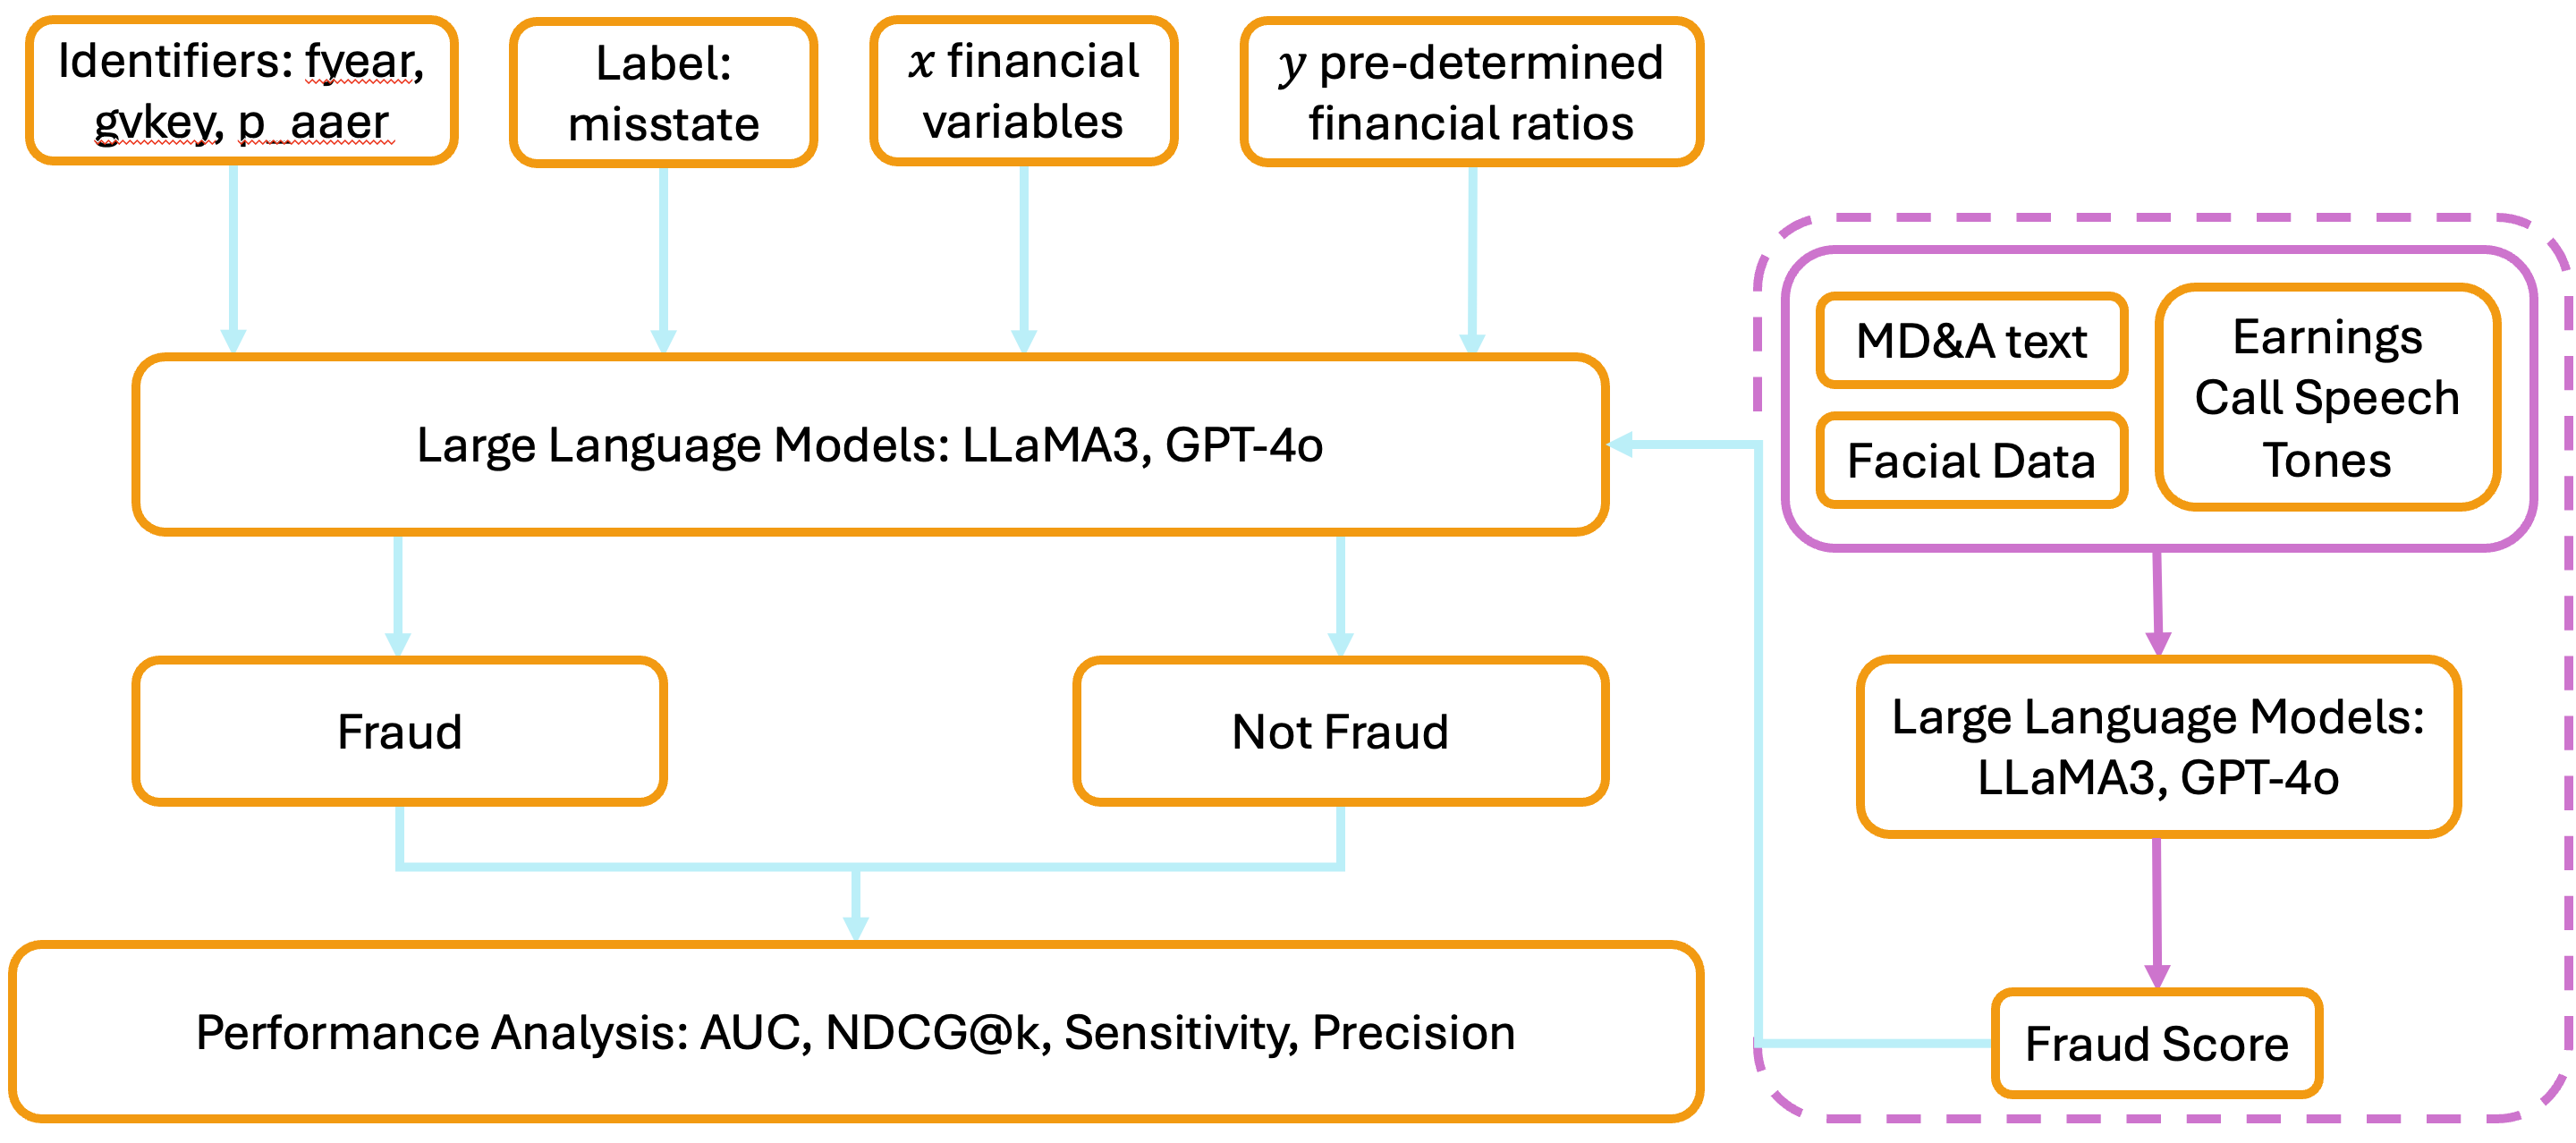
\includegraphics[width=\columnwidth]{llmmethod}}
	\caption{Figure of Future Experiments}
	\label{fig}
	\end{figure} \vspace{15pt}
\subsection{Dataset Expansion}
We plan to increase the dataset's scope into the current year of study, 2024. That would bring valuable training data and present an opportunity to test our fraud detection model on previously untested data. This would require lots of manual work by scraping off of the SEC AAERs webpage to update the dataset up until 2024, as the current dataset only goes until 2018. Additionally, we will leverage the Compustat database to fill in the financial variables for firms from 2018-2024. Once this dataset is complete, we hope to re-run the experiment and determine any improvements and hyperparameter tunings that can be made to the models. 

\subsection{Large-Language Models (LLMs)}
We plan to leverage LLMs to give a fraud score when given an input of financial statement text data (MD\&A, earnings call transcript). This will become another feature inputted into a baseline's preliminary machine learning methods. We aim to use the LLMs and see if we can achieve performance gains by inputting our financial variables, ratios, and text data. Similarly to our machine learning approach, the model will classify a firm as either fraudulent or non-fraudulent, and then a performance analysis will be conducted to see if the results have improved or worsened or stayed the same. We hope to implement GPT-4o and LLaMA3 following a similar methodology to Chen, Kelly, Xiu [2023] \cite{b2}, and improve upon our results and be able to publish a state-of-the-art fraud detection model using an LLM approach. Outside of this project's scope, we want to incorporate both speaking tones (speech detection) and facial expressions (computer vision) to increase the robustness of the dataset even more. 


\begin{thebibliography}{00}
\bibitem{b1} Cecchini, M.; H. Aytug; G. J. Koehler; AND P. Pathak. “Detecting Management Fraud in Public Companies.” Management Science 56 (2010): 1146–60.
\bibitem{b2} Chen, Yifei and Kelly, Bryan T. and Xiu, Dacheng, Expected Returns and Large Language Models (November 22, 2022). Available at SSRN: https://ssrn.com/abstract=4416687
\bibitem{b8} Cressey, D.R. (1973). Other Peoples’ Money: A study in the social psychology of embezzlement. Glencoe: Free Press.
\bibitem{b3} Dechow, P. M.;W. Ge; C. R. Larson; and R. G. Sloan. “Predicting Material Accounting Misstatements.”
Contemporary Accounting Research 28 (2011): 17–82.
\bibitem{b4} Dyck, A.; A. Morse; AND L. Zingales. “Who Blows the Whistle on Corporate Fraud?” Journal of Finance LXV (2010): 2213–53.
\bibitem{b9} Fawcett, T. “An Introduction to ROC Analysis.” Pattern Recognition Letters 27 (2006): 861–74.
\bibitem{b5} J. Gee, M. Button, The Financial Cost of Fraud 2019, Tech. Rep, Crowe, 2019.
\bibitem{b6} Rakoff, J. S. “The Financial Crisis: Why Have No High-Level Executives Been Prosecuted?”
The New York Review of Books, January 9, 2014.
\bibitem{b7} Yang Bao, Bin Ke, Bin Li, Julia Yu, and Jie Zhang (2020). Detecting Accounting Fraud in Publicly Traded U.S. Firms Using a Machine Learning Approach. Journal of Accounting Research, 58 (1): 199-235.
\end{thebibliography}

\newpage
\section*{Appendix}
\begin{table}[H]
\caption{Reported Evaluation Metrics for the Test Period 2003-08 \newline Input: 28 Financial Variables}
\centering
\begin{tabular}{p{2.495cm}cccc}
\toprule
\textbf{Method} & \textbf{AUC} & \textbf{NDCG@k} & \textbf{Sensitivity} & \textbf{Precision} \\
\midrule
\raggedright (1) Logit & 0.690 & 0.006 & 0.73\% & 0.85\% \\
\raggedright (2) RUSBoost & 0.725 & 0.049 & 4.88\% & 4.48\% \\
\raggedright (3) SVM & 0.680 & 0.016 & 1.69\% & 1.90\% \\
\bottomrule
\end{tabular}
\label{tab:performance}
\end{table}
\begin{table}[H]
\caption{Percentage Change From Table VII to Table IV}
\centering
\begin{tabular}{p{2.295cm}ccccc}
\toprule
\textbf{Method} & \textbf{AUC} & \textbf{NDCG@k} & \textbf{Sensitivity} & \textbf{Precision} \\
\midrule
\raggedright (1) Logit & -7.25\% & 350.00\% & 358.22\% & 234.71\% \\
\raggedright (2) RUSBoost & 6.21\% & 4.08\% & 1.70\% & 13.82\% \\
\raggedright (3) SVM & -6.18\% & 50.00\% & 80.89\% & 34.84\% \\

\bottomrule
\end{tabular}
\end{table}

\end{document}